% ------------------------------------------------------------------------------------------------ %
% ZUSAMMENFASSUNG
% WAHRSCHEINLICHKEIT UND STATISTIK
% ------------------------------------------------------------------------------------------------ %
% Autor: J�r�me Dohrau
% Email: dohrauj @ ...
% Die Zusammenfassung darf gerne f�r den eigenen Gebrauch angepasst werden. Falls jemand einen
% Fehler findet, w�rde ich mich �ber eine Benachrichtigung per Email freuen.
% ------------------------------------------------------------------------------------------------ %


\documentclass[a4paper,twocolumn]{article}


% ------------------------------------------------------------------------------------------------ %
% ALLGEMEINE PAKETE
% ------------------------------------------------------------------------------------------------ %


% Silbentrennung, Sonderzeichen ect.
\usepackage[german]{babel}
\usepackage[T1]{fontenc}

% Mathematische Zeichen
\usepackage{amssymb}
% Lehrs�tze
\usepackage{amsthm}
% Mathematische Extras (Matrizen ect.)
\usepackage{amsxtra}

% F�r kompakte Listen
\usepackage{paralist}

% Rahmen
\usepackage{framed}

% Grafik
\usepackage{graphicx}
\usepackage{ifpdf}
\usepackage{psfrag}
\usepackage{epstopdf}

\usepackage{titlesec}
\usepackage{titletoc}

% Graphs and Automata
\usepackage{gastex}

% farben
\usepackage{color}
\usepackage{bbold}


% ------------------------------------------------------------------------------------------------ %
% FARBEN
% ------------------------------------------------------------------------------------------------ %


\definecolor{headtext}{rgb}{0.50,0.50,0.50}
\definecolor{foottext}{rgb}{0.50,0.50,0.50}
\definecolor{headsepline}{rgb}{0.80,0.80,0.80}
\definecolor{footsepline}{rgb}{0.80,0.80,0.80}


% Schattierung f�r Hinweisboxen
\definecolor{shadecolor}{rgb}{0.88,0.91,0.95}

\definecolor{highlightcolor}{rgb}{1.00,0.50,0.50}


% ------------------------------------------------------------------------------------------------ %
% SEITEN- UND TEXTLAYOUT
% ------------------------------------------------------------------------------------------------ %


% Seitenr�nder
\usepackage[left=10mm,right=10mm,top=20mm,bottom=20mm]{geometry}

% Zeileneinzug am Anfang eines Absatzes
\setlength{\parindent}{0em}


% ------------------------------------------------------------------------------------------------ %
% KOPF- UND FUSSZEILEN
% ------------------------------------------------------------------------------------------------ %


\usepackage{fancyhdr}
\pagestyle{fancy}

\fancyhead{} % l�schen
\fancyhead[L]{\color{headtext}\uppercase{Wahrscheinlichkeit und Statistik}}
\fancyhead[R]{\color{headtext}\leftmark}

\fancyfoot{} % l�schen
\fancyfoot[L]{\color{foottext}\uppercase{Seite} \thepage}
\fancyfoot[R]{\color{foottext}\uppercase{Jerome Dohrau}}

\renewcommand{\headrulewidth}{1pt}
\renewcommand{\headrule}{{\color{headsepline}\hrule width\headwidth height\headrulewidth \vskip-\headrulewidth}}
\renewcommand{\footrulewidth}{1pt}
\renewcommand{\footrule}{{\color{footsepline}\vskip-\footruleskip\vskip-\footrulewidth\hrule width\headwidth height\footrulewidth\vskip\footruleskip}}


% ------------------------------------------------------------------------------------------------ %
% LEHRS�TZE (DEFINITIONEN ETC.)
% ------------------------------------------------------------------------------------------------ %


\newtheoremstyle{defstyle}
	% Abstand oben
	{10pt}
	% Abstand unten
	{10pt}
	% Schriftart
	{\normalfont}
	% Zeileneinzug (leer = kein Zeileneinzug, \parindent = Absatz-Zeileneinzug)
	{}
	% Titel Schriftart
	{\normalfont\bfseries}
	% Zeichen nach dem Titel
	{:} 
	% Leerraum nach dem Titel
	{ }
	% Lehrsatzkopf definieren (leer = normal)
	{#3}

\newtheoremstyle{thmstyle}
	% Abstand oben
	{10pt}
	% Abstand unten
	{10pt}
	% Schriftart
	{\normalfont}
	% Zeileneinzug (leer = kein Zeileneinzug, \parindent = Absatz-Zeileneinzug)
	{}
	% Titel Schriftart
	{\normalfont\bfseries}
	% Zeichen nach dem Titel
	{:} 
	% Leerraum nach dem Titel
	{ }
	% Lehrsatzkopf definieren (leer = normal)
	{\thmname{#1}\thmnumber{ #2}\thmnote{ (#3)}}

\theoremstyle{defstyle}
% Definition
\newtheorem*{definition}{Definition}

\theoremstyle{thmstyle}
% 
\newtheorem*{theorem}{Satz}
% Beachte
\newtheorem*{tnote}{Hinweis}

% Beispiel
\newtheorem*{example}{Beispiel}

\newenvironment{note}
	{\begin{snugshade}\begin{tnote}}
	{\end{tnote}\end{snugshade}}
	
\newenvironment{highlight}
	{\begin{snugshade}}
	{\end{snugshade}}


% ------------------------------------------------------------------------------------------------ %
% ABBILDUNGEN
% ------------------------------------------------------------------------------------------------ %


\usepackage[bf]{caption}

\addto\captionsgerman{
    \renewcommand{\figurename}{Abb.}
    \renewcommand{\tablename}{Tab.}}

% Abbildungs�berschrift
\renewcommand{\captionfont}{\footnotesize\sffamily}


% ------------------------------------------------------------------------------------------------ %
% SELBSTDEFINIERTE BEFEHLE
% ------------------------------------------------------------------------------------------------ %


\newcommand{\todo}[1]{{\definecolor{shadecolor}{rgb}{1.00,0.30,0.30}\begin{snugshade}{\bf TODO:} #1\end{snugshade}}}

\newcommand{\R}{\mathbb{R}}
\newcommand{\N}{\mathbb{N}}
\renewcommand{\P}{\mathbb{P}}
\newcommand{\E}{\mathbb{E}}

\renewcommand{\d}{\mathrm{d}}

\renewcommand{\theta}{\vartheta}
\renewcommand{\phi}{\varphi}

\newcommand{\var}{\mathrm{Var}}
\newcommand{\cov}{\mathrm{Cov}}
\newcommand{\sd}{\mathrm{sd}}
\newcommand{\corr}{\mathrm{Corr}}

\newcommand{\abs}[1]{\lvert #1 \rvert}


% ------------------------------------------------------------------------------------------------ %
% LAYOUT INHALTSVERZEICHNIS UNDSO
% ------------------------------------------------------------------------------------------------ %


\renewcommand{\thepart}{\Alph{part}}
\renewcommand{\thesection}{\Alph{part}.\arabic{section}}

\titlecontents{part}[0em]%
{\vspace{1em}\bf\large}{\thecontentslabel\enskip}{}%
{\hfill\contentspage}

\titlecontents{section}[0em]%
{\vspace{0.3em}\bf}{\thecontentslabel\enskip}{}%
{\hfill\contentspage}

\titlecontents{subsection}[1em]%
{}{\thecontentslabel\enskip}{}%
{\titlerule*[0.6em]{.}\contentspage}

\titlecontents{subsubsection}[2em]%
{}{\thecontentslabel\enskip}{}%
{\titlerule*[0.6em]{.}\contentspage}


% ------------------------------------------------------------------------------------------------ %
% INHALT
% ------------------------------------------------------------------------------------------------ %


\begin{document}

\setcounter{tocdepth}{2}
\tableofcontents

\hfill\newpage

\setcounter{part}{23}
\part*{Wahrscheinlichkeit}
\addcontentsline{toc}{part}{Wahrscheinlichkeit}

% ------------------------------------------------------------------------------------------------ %
% GRUNDLAGEN
% ------------------------------------------------------------------------------------------------ %

\section{Wahrscheinlichkeiten}


% ------------------------------------------------------------------------------------------------ %
% Ereignissraum
% ------------------------------------------------------------------------------------------------ %


\subsection{Ereignisraum, Grundraum}

\begin{definition}[Ereignisraum]
Der \emph{Ereignisraum} oder \emph{Grundraum} $\Omega$ ist die Menge aller m�glichen Ereignisse eines Zufallexperiments. Die Elemente $\omega \in \Omega$ heissen \emph{Elementarereignisse}.
\end{definition}

\begin{definition}[Ereignis]
Ein \emph{Ereignis} $A \subseteq \Omega$ ist eine Teilmenge von $\Omega$.
\end{definition}

Die Klasse aller \emph{beobachtbaren Ereignisse} $\mathcal{F}$ ist eine Teilmenge der Potenzmenge $\mathcal{P}(\Omega)$ von $\Omega$.


% ------------------------------------------------------------------------------------------------ %
% Das Wahrscheinlichkeitsmass
% ------------------------------------------------------------------------------------------------ %


\subsection{Wahrscheinlichkeitsmass}

\begin{definition}[Wahrscheinlichkeitsmass]
Ein \emph{Wahrscheinlichkeitsmass} $\P$ ist eine Abbildung $\P:\mathcal{F} \rightarrow [0,1]$ mit folgenden Eigenschaften:
\begin{compactenum}[i:]
\item $\P[\Omega] = 1$.
\item $\P[A] \geq 0$ f�r alle $A \in \mathcal{F}$.
\item $\P[\bigcup_{i=1}^\infty A_i] = \sum_{i=1}^\infty \P[A_i]$ falls $A_i \cap A_j = \emptyset$ f�r $i \neq j$.
\end{compactenum}
\end{definition}

Aus den Axiomen i bis iii folgen direkt die Rechenregeln:
\begin{compactenum}[i:]
\item $\P[A^C] = 1 - \P[A]$.
\item $\P[\emptyset] = 0$.
\item $A \subseteq B \Rightarrow \P[A] \leq \P[B]$.
\item $\P[A \cup B] = \P[A]+\P[B]-\P[A \cap B]$ (\emph{Additionsregel}).
\end{compactenum}


% ------------------------------------------------------------------------------------------------ %

\subsection{Endliche R�ume}

F�r einen endlichen Raum $\Omega = \{\omega_1,\ldots,\omega_n\}$ mit $\P[\omega_i] = p_i$ f�r alle $1 \leq i \leq n$ gilt
$$
\P[A] = \sum_{ i \text{ mit } w_i \in A} p_i
$$


\begin{definition}[Laplace-Raum]
In einem \emph{Laplace-Raum} sind alle Ereignisse $\omega_1,\ldots,\omega_n$ gleich wahrscheinlich ($p_i = p_j$ f�r alle $i,j$). Es gilt dann
$$
P[A] = \frac{\lvert A \rvert}{\lvert \Omega \rvert}
$$
\end{definition}


% ------------------------------------------------------------------------------------------------ %
% BEDINGTE WAHRSCHEINLICHKEIT, TOTALE WAHRSCHEINLICHKEIT UND FORMEL VON BAYES
% ------------------------------------------------------------------------------------------------ %


\subsection{Bedingte Wahrscheinlichkeit}

\begin{definition}[Bedingte Wahrscheinlichkeit]
Seien $A,B$ Ereignisse und $\P[A] > 0$, dann ist die \emph{bedingte Wahrscheinlichkeit} von $B$ gegeben $A$ definiert durch:
$$
\P[B \mid A] := \frac{\P[A \cap B]}{\P[A]}
$$
\end{definition}

Aus der Definition der bedingten Wahrscheinlichkeit folgt die \emph{Multiplikationsregel}:
$$
\P[A \cap B] = \P[B \mid A] \P[A]
$$

\begin{theorem}[Totale Wahrscheinlichkeit]
Sei $A_{1 \leq i \leq n}$ eine disjunkte Zerlegung von $\Omega$, dann gilt f�r ein beliebiges Ereignis $B$:
$$
\P[B] = \sum_{i=1}^n \P[B \mid A_i]\P[A_i]
$$
\end{theorem}

\begin{theorem}[Formel von Bayes]
Sei $A_1,\ldots,A_n$ eine disjunkte Zerlegung von $\Omega$ mit $\P[A_i] > 0$ f�r alle $i$ und $B$ ein Ereignis mit $\P[B] > 0$, dann gilt f�r jedes $k$:
$$
\P[A_k \mid B] = \frac{\P[B \mid A_k] \P[A_k]}{\sum_{i=1}^n \P[B \mid A_i] \P[A_i]}
$$
\end{theorem}


% ------------------------------------------------------------------------------------------------ %
% UNABH�NGIGKEIT
% ------------------------------------------------------------------------------------------------ %


\subsection{Unabh�ngigkeit}

\begin{definition}[Unabh�ngigkeit]
Die Ereignisse $A_1,\ldots,A_n$ heissen \emph{unabh�ngig}, wenn f�r alle $m \in \N$ und $\{k_1,\ldots,k_m\} \subseteq \{1,\ldots,n\}$ gilt

$$
\P\left[\bigcap_{i=1}^m A_{k_i}\right] = \prod_{i=1}^m \P[A_{k_i}].
$$
\end{definition}

\begin{note}
Bei unabh�ngigen Ereignissen $A,B$ hat das Eintreten des einen Ereignisses keinen Einfluss auf die Wahrscheinlichkeit des anderen Ereignisses: $\P[B \mid A] = \frac{\P[A \cap B]}{\P[A]} = \P[B]$
\end{note}


% ------------------------------------------------------------------------------------------------ %
% ------------------------------------------------------------------------------------------------ %
% Zufallsvariablen
% ------------------------------------------------------------------------------------------------ %


\section{Zufallsvariablen}

\begin{definition}[Zufallsvariable]
Eine \emph{Zufallsvariable} $X$ auf $\Omega$ ist eine Funktion $X:\Omega \rightarrow \mathcal{W}(X) \subseteq \R$. Jedes Elementarereignis $\omega$ wird auf eine Zahl $X(\omega)$ abgebildet.
\end{definition}

\begin{definition}[Verteilungsfunktion]
Die \emph{Verteilungsfunktion} einer Zufallsvariable $X$ ist die Abbildung $F_X:\R \rightarrow[0,1]$,
$$
F_X(t) := \P[X \leq t] := \P[\{\omega \mid X(\omega) \leq t\}].
$$
\end{definition}

Jede Verteilungsfunktion $F_X$ hat folgende Eigenschaften:
\begin{compactenum}[i:]
\item $a \leq b \Rightarrow F_X(a) \leq F_X(b)$ (monoton wachsend).
\item $\displaystyle\lim_{t\rightarrow u, t > u}F_X(t) = F_X(u)$ (rechtsstetig).
\item $\displaystyle\lim_{t\rightarrow-\infty} F_X(t) = 0$ und $\displaystyle\lim_{t\rightarrow\infty} F_X(t) = 1$.
\end{compactenum}


% ------------------------------------------------------------------------------------------------ %
% Diskrete Zufallsvariablen
% ------------------------------------------------------------------------------------------------ %


\subsection{Diskrete Zufallsvariablen}

Eine Zufallsvariable heisst \emph{diskret}, falls ihr Wertebereich $\mathcal{W}(X)$ endlich oder abz�hlbar ist.

\begin{definition}[Gewichtsfunktion]
Die \emph{Wahrscheinlichkeitsfunktion} oder \emph{Gewichtsfunktion} einer diskreten Zufallsvariable $X$ ist gegeben durch
$$
p_X(x) =
\left\{\begin{array}{ll}
\P[X = x] & \text{f�r }x \in \mathcal{W}(X) \\
0         & \text{sonst}
\end{array}\right.
$$
\end{definition}

Eine Gewichtsfunktion weist folgende Eigenschaften auf:
\begin{compactenum}[i:]
\item $p_X(x) \in [0,1]$ f�r alle $x$.
\item $\sum_{x_i \in \mathcal{W}(X)} p_X(x_i) = 1$.
\end{compactenum}

\begin{definition}[Diskrete Verteilungsfunktion]
Die Verteilungsfunktion $F_X$ einer diskreten Zufallsvariable $X$ mit Wertebereich $\mathcal{W}(X) = \{x_1,\ldots,x_n\}$ ist die Funktion
$$
F_X(t) =
\P[X \leq t] =
\sum_{x_k \in \mathcal{W}(X) \atop x_k \leq t} p_X(x_k)
$$
\end{definition}


% ------------------------------------------------------------------------------------------------ %
% Stetige zufallsvariablen
% ------------------------------------------------------------------------------------------------ %


\subsection{Stetige Zufallsvariablen}

\begin{definition}[Dichte]
Eine Zufallsvariable $X$ mit der Verteilungsfunktion $F_X(t)$ heisst stetig mit \emph{Dichte} $f_X:\R\rightarrow[0,\infty)$, falls gilt
$$
F_X(t) = \int_{-\infty}^t f_X(s) \d s
\quad
\text{f�r alle } t \in \R.
$$
\end{definition}

F�r eine Dichtefunktion $f_X$ gilt:
\begin{compactenum}[i:]
\item $f_X(t) \geq 0$ f�r alle $t \in \R$.
\item $\int_{-\infty}^\infty f_X(s) \d s = 1$.
\end{compactenum}

\begin{note}
Es gilt $\frac{\d}{\d t} F_X(t) = f_X(t)$ falls $f_X$ an der Stelle $t$ stetig ist.
\end{note}


% ------------------------------------------------------------------------------------------------ %
% TRANSFORMATION
% ------------------------------------------------------------------------------------------------ %


\subsection{Transformation von Zufallsvariablen}

\begin{theorem}
Sei $X$ eine stetige Zufallsvariable mit Dichte $f_X$ und $f_X(t) = 0$ f�r $t \notin I \subseteq \R$. Sei $g:\R\rightarrow\R$ stetig differenzierbar und streng monoton auf $I$ mit Umkehrfunktion $g^{-1}$. Dann hat die Zufallsvariable $Y := g(X)$ die Dichte
$$
f_Y =
\left\{\begin{array}{ll}
f_X (g^{-1}(t)) \lvert\frac{\d}{\d t} g^{-1}(t)\rvert & \text{f�r } t \in \{g(x) \mid x \in I\} \\[1ex]
0 & \text{sont}
\end{array}\right.
$$
\end{theorem}

\begin{example}[Lineare Transformation] Aus $Y := aX+b$ mit $a>0,b \in\R$ folgt
$$
F_Y(t) =
\P[aX+b \leq t] =
\P\left[X \leq \frac{t-b}{a}\right] =
F_X\left(\frac{t-b}{a}\right)
$$
und mit der Kettenregel ergibt sich
$$
f_Y(t) = \frac{\d}{\d t}F_Y(t) = \frac{1}{a} f_X\left(\frac{t-b}{a}\right).
$$
\end{example}

\begin{example}[Nichtlineare Transformation] Aus $Y := X^2$ folgt
$$
F_Y(t) =
\P[X^2 \leq t] =
\P\bigl[-\sqrt{t} \leq X \leq \sqrt{t}\bigr] =
F_X\bigl(\sqrt{t}\bigr)-F_X\bigl(-\sqrt{t}\bigr)
$$
und somit
$$
f_Y(t) = \frac{\d}{\d t}F_Y(t) =
\frac{f_X\bigl(\sqrt{t}\bigr)+f_X\bigl(-\sqrt{t}\bigr)}{2\sqrt{t}}
$$
\end{example}


% ------------------------------------------------------------------------------------------------ %
% SIMULATION VON VERTEILUNGEN
% ------------------------------------------------------------------------------------------------ %

\subsection{Simulation von Verteilungen}

\begin{theorem}
Sei $F$ eine stetige und streng monoton wachsende Verteilungsfunktion mit Umkehrfunktion $F^{-1}$. Ist $X \sim \mathcal{U}(0,1)$ und $Y := F^{-1}(X)$, so hat $Y$ die Verteilungsfunktion $F$.
\end{theorem}

\begin{example} Um die Verteilung $Exp(\lambda)$ zu simulieren bestimmt man zu der Verteilungsfunktion $F(t) = 1-e^{-\lambda t}$ f�r $t \geq 0$ die Inverse $F^{-1}(t) = -\frac{\log(1-t)}{\lambda}$. Mit $U \sim \mathcal{U}(0,1)$ erh�lt man
$$
X := F^{-1}(U) = -\frac{\log(1-U)}{\lambda} \sim Exp(\lambda).
$$
\end{example}

% ------------------------------------------------------------------------------------------------ %
% ------------------------------------------------------------------------------------------------ %
% Erwartungswert
% ------------------------------------------------------------------------------------------------ %


\subsection{Erwartungswert}

\begin{definition}[Diskreter Erwartungswert]
Ist $X$ diskrete Zufallsvariable mit Gewichtsfunktion $p_X$, so ist der \emph{Erwartungswert} von $X$ definiert als
$$
\E[X] := \sum_{x_i \in \mathcal{W}(X)} x_i p_X(x_i),
$$
sofern diese Reihe konvergiert.
\end{definition}

\begin{definition}[Stetiger Erwartungswert]
Falls $X$ eine stetige Zufallsvariable mit Dichte $f_X$ ist, dann ist der \emph{Erwartungswert} von $X$ definiert als
$$
\E[X] := \int_{-\infty}^\infty x f_X(x) \d x,
$$
falls das Integral konvergiert.
\end{definition}

\begin{theorem}[4.1]
Sei $X$ eine diskrete Zufallsvariable mit Gewichtsfunktion $p_X$ und $Y := g(X)$, dann gilt
$$
\E[Y] = \E[g(X)] = \sum_{x_i \in \mathcal{W}(X)} g(x_i) p_{X}(x_i).
$$
Falls $X$ eine stetige Zufallsvariable mit Dichte $f_X$ ist, ist analog
$$
\E[Y] = \E[g(X)] = \int_{-\infty}^\infty g(x) f_X(x) \d x
$$
\end{theorem}


% ------------------------------------------------------------------------------------------------ %
% VARIANZ UND STANDARDABWEICHUNG
% ------------------------------------------------------------------------------------------------ %

\subsection{Varianz und Standardabweichung}

\begin{definition}[Varianz]
Sei $X$ eine Zufallsvariable mit $\E[X^2] < \infty$. Die \emph{Varianz} von $X$ ist definiert als
$$
\var[X] := \E\left[(X-\E(X))^2\right].
$$
\end{definition}

\begin{note} Nach Satz 4.1 l�sst sich die Varianz folgendermassen berechnen:
$$
\var[X] = \int_{-\infty}^\infty (x-\E[X])^2 f_X(x) \d x
$$
\end{note}

\begin{definition}[Standardabweichung]
Die \emph{Standardabweichung} einer Zufallsvariable $X$ ist
$$
\sigma_X := \sqrt{\var[X]}.
$$
\end{definition}


% ------------------------------------------------------------------------------------------------ %
% ------------------------------------------------------------------------------------------------ %


\section{Wichtige Verteilungen}


% ------------------------------------------------------------------------------------------------ %
% DISKRETE VERTEILUNGEN
% ------------------------------------------------------------------------------------------------ %


\subsection{Diskrete Verteilungen}


% ------------------------------------------------------------------------------------------------ %
% DISKRETE GLEICHVERTEILUNG
% ------------------------------------------------------------------------------------------------ %


\subsubsection{Diskrete Gleichverteilung}

Zufallsvariable $X$ mit Wertebereich $\mathcal{W}(X) = \{x_1,\ldots,x_n\}$ und alle Werte haben die gleiche Wahrscheinlichkeit falls
$$
p_X(x_i) = \frac{1}{n}
\quad
\text{f�r } i \in \{1,\ldots,n\}
$$

\begin{example}[W�rfeln] Die Zufallsvariable $X$ gibt die Augenzahl bei einem W�rfelwurf an. Der Wertebereich ist also
$\mathcal{W} = \{1,2,3,4,5,6\}$ und somit $n=6$.
\end{example}


% ------------------------------------------------------------------------------------------------ %
% BERNOULLI VERTEILUNG
% ------------------------------------------------------------------------------------------------ %


\subsubsection{Bernoulli-Verteilung}

Eine bernoulli-verteilte Zufallsvariable $X \sim Be(p)$ mit Parameter $p \in [0,1]$ nimmt die Werte $0$ und $1$ mit Wahrscheinlichkeiten
$$
p_X(1) = p
\quad\text{und}\quad
p_X(0) = 1-p
$$
an. Eine alternative Schreibweise ist
$$
p_X(x) =
\left\{\begin{array}{ll}
p^x (1-p)^{1-x} & x \in \{0,1\} \\
0 & \text{sonst}.
\end{array}\right.
$$

\begin{highlight}
\begin{tabular}{l@{ : }l}
Erwartungswert & $p$ \\
Varianz        & $p(1-p)$
\end{tabular}
\end{highlight}

\begin{example}[M�nzwurf] Ein fairer M�nzwurf ist bernoulli-verteilt mit Parameter $p=\frac{1}{2}$. F�r einen Parameter $p \neq \frac{1}{2}$ w�re der M�nzwurf unfair.
\end{example}


% ------------------------------------------------------------------------------------------------ %
% BINOMIALVERTEILUNG
% ------------------------------------------------------------------------------------------------ %


\subsubsection{Binomialverteilung}

Die Gewichtsfunktion $p_X$ einer binomial-verteilten Zufallsvariable $X \sim Bin(n,p)$ mit Parameter $n \in \N$ und $p \in [0,1]$ ist gegeben durch
$$
p_x(k) = {n \choose k} p^k (1-p)^{n-k}
\quad
\text{f�r } k \in \{0,\ldots,n\}
$$

\begin{highlight}
\begin{tabular}{l@{ : }l}
Erwartungswert & $np$ \\
Varianz        & $np(1-p)$
\end{tabular}
\end{highlight}

$X$ ist die Anzahl der Erfolge $k$ bei $n$ unabh�ngigen Wiederholungen eines Bernoulli-Experiments. Es gibt ${n \choose k}$ verschiedene M�glichkeiten bei $n$ Versuchen $k$-mal erfolgreich zu sein. Jeder dieser M�glichkeit hat Wahrscheinlichkeit $p^k (1-p)^{n-k}$.


% ------------------------------------------------------------------------------------------------ %
% GEOMETRISCHE VERTEILUNG
% ------------------------------------------------------------------------------------------------ %


\subsubsection{Geometrische Verteilung}

Die Gewichtsfunktion $p_X$ einer geometrisch-gleichverteilten Zufallsvariable $X \sim Geom(p)$  mit Parameter $p \in [0,1]$ ist gegeben durch
$$
p_X(k) = p(1-p)^{k-1}
\quad
\text{f�r } k \in \{1,2,\ldots\}
$$

\begin{highlight}
\begin{tabular}{l@{ : }l}
Erwartungswert & $\frac{1}{p}$ \\
Varianz        & $\frac{1}{p^2}(1-p)$
\end{tabular}
\end{highlight}

\begin{example}[Wartezeit] Die Geometrische Verteilung ist die Wahrscheinlichkeitsverteilung der Anzahl $X$ Bernoulli-Versuche, die notwendig sind, um den ersten Erfolg zu erzielen. F�r die Anzahl W�rfelfw�rfe, die man braucht um eine $6$ zu w�rfeln, ist $p = \frac{1}{6}$.
\end{example}


% ------------------------------------------------------------------------------------------------ %
% NEGATIVBINOMIALE VERTEILUNG
% ------------------------------------------------------------------------------------------------ %


\subsubsection{Negativbinomiale Verteilung}

Die Gewichtsfunktion $p_X$ einer negativ-binomial-verteilten Zufallsvariable $X$ mit Parameter $r \in \N$ und $p \in [0,1]$ ist gegeben durch
$$
p_X(k) = {{k-1} \choose {r-1}}p^r(1-p)^{k-r}
\quad
\text{f�r } k \in \{r,r+1,\ldots\}
$$

\begin{highlight}
\begin{tabular}{l@{ : }l}
Erwartungswert & $\frac{r}{p}$ \\
Varianz        & $\frac{r}{p^2}(1-p)$
\end{tabular}
\end{highlight}

$X$ entspricht der Wartezeit auf den $r$-ten Erfolg. Es gibt ${{k-1} \choose {r-1}}$ m�glichkeiten f�r $r-1$ Erfolge bei $k-1$ Versuchen; der $r$-te Erfolg tritt ja beim $k$-ten Versuch ein.


% ------------------------------------------------------------------------------------------------ %
% HYPERGEOMETRISCHE VERTEILUNG
% ------------------------------------------------------------------------------------------------ %


\subsubsection{Hypergeometrische Verteilung}

Die Gewichtsfunktion $p_X$ einer hypergeometrisch-verteilten Zufallsvariable $X$ mit Parameter $r,n,m \in \N$, wobei $r,m \leq n$, ist gegeben durch
$$
p_X(k) = \frac{{r \choose k}{{n-r} \choose {m-k}}}{{n \choose m}}
\quad
\text{f�r } k \in \{0,\ldots,\min\{r,m\}\}
$$

\begin{highlight}
\begin{tabular}{l@{ : }l}
Erwartungswert & $m\frac{r}{n}$ \\
Varianz        & $m\frac{r}{n}(1-\frac{r}{n})\frac{n-m}{n-1}$
\end{tabular}
\end{highlight}

In einer Urne befinden sich $n$ Gegenst�nde. Davon sind $r$ Gegenst�nde vom Typ A und $n-r$ vom Typ B. Es werden $m$ Gegenst�nde ohne Zur�cklegen gezogen. $X$ beschreibt die Wahrscheinlichkeitsverteilung f�r die Anzahl $k$ der Gegenst�nde vom Typ A in der Stichprobe.

\begin{example}[Lotto]
Anzahl Zahlen $n=45$, richtige Zahlen $r=6$, meine Zahlen $m=6$. Die Wahrscheinlichkeit f�r $4$ Richtige ist
$$
p_X(4) = \frac{{6 \choose 4}{39 \choose 2}}{{45 \choose 6}} \approx 0.00136.
$$
\end{example}


% ------------------------------------------------------------------------------------------------ %
% POISSONVERTEILUNG
% ------------------------------------------------------------------------------------------------ %


\subsubsection{Poisson Verteilung}

Die Gewichtsfunktion $p_X$ einer Poisson-verteilten Zufallsvariable $X \sim \mathcal{P}(\lambda)$ mit Parameter $\lambda$ ist gegeben durch
$$
p_X(k) = e^{-\lambda}\frac{\lambda^k}{k!}
\quad
\text{f�r } k \in \{0,1,\ldots\}
$$

\begin{highlight}
\begin{tabular}{l@{ : }l}
Erwartungswert & $\lambda$ \\
Varianz        & $\lambda$
\end{tabular}
\end{highlight}

Die Poisson-Verteilung eignet sich zur Modellierung von seltenen Ereignissen, wie z.B. Versicherungssch�den.

\begin{note}
Die Binomialverteilung $Bin(n,p)$ kann approximativ durch die Poissonverteilung $\mathcal{P}(\lambda)$ mit $\lambda = np$ berechnet werden.
Faustregel: Die Approximation kann f�r $np^2 \leq 0.05$ benutzt werden.
\end{note}


% ------------------------------------------------------------------------------------------------ %
% STETIGE VERTEILUNGEN
% ------------------------------------------------------------------------------------------------ %


\subsection{Stetige Verteilungen}


% ------------------------------------------------------------------------------------------------ %
% STETIGE GLEICHVERTEILUNG
% ------------------------------------------------------------------------------------------------ %


\subsubsection{Stetige Gleichverteilung}
Die Dichte $f_X$ und Verteilungsfunktion $F_X$ einer stetigen und gleichverteilten Zufallsvariable $X \sim \mathcal{U}(a,b)$ mit Parameter $a,b \in \R$ wobei $a < b$ sind gegeben durch
$$
\begin{array}{rcl}
f_X(t) & = &
\left\{\begin{array}{ll}
\frac{1}{b-a} & \text{f�r } t \in [a,b] \\[1ex]
0             & \text{f�r } t \notin [a,b]
\end{array}\right.
\\[1.5em]
F_X & = &
\left\{\begin{array}{ll}
0               & \text{f�r } t < a \\[1ex]
\frac{t-a}{b-a} & \text{f�r } t \in [a,b] \\[1ex]
1               & \text{f�r } t > b
\end{array}\right.
\end{array}
$$

\begin{highlight}
\begin{tabular}{l@{ : }l}
Erwartungswert & $\frac{1}{2}(a+b)$ \\
Varianz        & $\frac{1}{12}(a-b)^2$
\end{tabular}
\end{highlight}

\begin{example}
Rundungsfehler einer Messung.
\end{example}

% ------------------------------------------------------------------------------------------------ %
% EXPONENTIALVERTEILUNG
% ------------------------------------------------------------------------------------------------ %


\subsubsection{Exponentialverteilung}

Die Dichte $f_X$ und Verteilungsfunktion $F_X$ einer exponential-verteilten Zufallsvariable $X \sim Exp(\lambda)$ mit Parameter $\lambda > 0$ sind gegeben durch
$$
\begin{array}{rcl}
f_X(t) & = & 
\left\{\begin{array}{ll}
\lambda e^{-\lambda t} & \text{f�r } t \geq 0 \\[1ex]
0                      & \text{f�r } t < 0
\end{array}\right.
\\[1.5em]
F_X(t) & = &
\left\{\begin{array}{ll}
1 - e^{-\lambda t} & \text{f�r } t \geq 0 \\[1ex]
0                  & \text{f�r } t < 0
\end{array}\right.
\end{array}
$$

\begin{highlight}
\begin{tabular}{l@{ : }l}
Erwartungswert & $\frac{1}{\lambda}$ \\
Varianz        & $\frac{1}{\lambda^2}$
\end{tabular}
\end{highlight}

\begin{example}[Lebensdauer]
Die Exponentialverteilung ist eine typische Lebensdauerverteilung. So ist beispielsweise die Lebensdauer von elektronischen Bauelementen h�ufig ann�hernd exponentialverteilt.
\end{example}


% ------------------------------------------------------------------------------------------------ %
% Normalverteilung
% ------------------------------------------------------------------------------------------------ %


\subsubsection{Normalverteilung}

Die Dichte $f_X$ einer normalverteilten Zufallsvariable $X \sim \mathcal{N}(\mu,\sigma^2)$ mit Parameter $\mu \in \R$ und $\sigma^2 > 0$ ist gegeben durch
$$
f_X(t) =
\frac{1}{\sigma\sqrt{2\pi}} \, e^{-\frac{(t-\mu)^2}{2\sigma^2}}
$$
F�r die Verteilungsfunktion $F_X$ existiert kein geschlossener Ausdruck. Deshalb werden die Werte der Verteilungsfunktion $\Phi(t)$ der \emph{Standard-Normalverteilung}
$$
f_X(t) =
\frac{1}{\sqrt{2\pi}} \, e^{-\frac{t^2}{2}}
$$
mit $\mu=0$ und $\sigma^2=1$ tabelliert. F�r allgemeine Normalverteilungen berechnet man dann
$$
F_X(t) = \P[X \leq t] = \P\left[\frac{X-\mu}{\sigma}\leq\frac{t-\mu}{\sigma}\right] = \Phi\left(\frac{t-\mu}{\sigma}\right).
$$

\begin{highlight}
\begin{tabular}{l@{ : }l}
Erwartungswert & $\mu$ \\
Varianz        & $\sigma^2$
\end{tabular}
\end{highlight}

\begin{example}
Streuung von Messwerten um den Mittelwert.
\end{example}


% ------------------------------------------------------------------------------------------------ %
% ------------------------------------------------------------------------------------------------ %
% GEMEINSAME UND BEDINGTE WAHRSCHEINLICHKEITEN
% ------------------------------------------------------------------------------------------------ %


\section{Gemeinsame Verteilungen}

\begin{definition}[Gemeinsame Verteilung]
Die \emph{gemeinsame Verteilungsfunktion} von $n$ Zufallsvariablen $X_1,\ldots,X_n$ ist die Abbildung $F:\R^n \rightarrow [0,1]$,
$$
F(t_1,\ldots,t_n) := \P[X_1 \leq t_1,\ldots,X_n \leq t_n].
$$
\end{definition}

\begin{definition}[Gemeinsame Gewichtsfunktion]
Falls $X_1,\ldots,X_n$ diskrete Zufallsvariablen sind, ist ihre \emph{gemeinsame Gewichtungsfunktion} $p:\R^n\rightarrow [0,1]$ definiert durch
$$
p(x_1,\ldots,x_n) := \P[X_1=x_1,\ldots,X_n=x_n].
$$
\end{definition}

\begin{definition}[Gemeinsame Dichte]
Seien $X_1,\ldots,X_n$ stetige Zufallsvariablen mit gemeinsamer Verteilungsfunktion $F(t_1,\ldots,t_n)$. Die Funktion $f : \R^n \rightarrow [0,\infty)$ heisst \emph{gemeinsame Dichte} von $X_1,\ldots,X_n$, falls f�r alle $t_i \in \R$ gilt
$$
F(t_1,\ldots,t_n) = \int_{-\infty}^{t_1} \ldots \int_{-\infty}^{t_n} f(x_1,\ldots,x_n) \d x_n \ldots \d x_1
$$
\end{definition}

Falls $X_1,\ldots,X_n$ eine gemeinsame Dichte $f$ haben, so hat diese folgende Eigenschaften:
\begin{compactenum}[i:]
\item $f(t_1,\ldots,t_n) \geq 0$ f�r alle $t_i \in \R$.
\item $\int_{\R^n} f(t_1,\ldots,t_n) \d\mu = 1$.
\item $\P[(X_1,\ldots,X_n) \in A] = \int_{(t_1,\ldots,t_n)\in A} f(t_1,\ldots,t_n) \d\mu$.
\item $f(t_1,\ldots,t_n) = \frac{\partial^n}{\partial t_1 \cdots \partial t_n} F(t_1,\ldots,t_n)$, falls definiert.
\end{compactenum}


% ------------------------------------------------------------------------------------------------ %
% RANDVERTEILUNG
% ------------------------------------------------------------------------------------------------ %


\subsection{Randverteilungen}

\begin{definition}[Randverteilung]
Seien $X$ und $Y$ Zufallsvariablen mit gemeinsamer Verteilungsfunktion $F_{X,Y}$, dann ist die \emph{Randverteilung} $F_X:\R \rightarrow [0,1]$ von $X$ definiert durch
$$
F_X := \P[X \leq x] = \P[X \leq x, Y < \infty] = \lim_{y\rightarrow\infty}F_{X,Y}(x,y).
$$
\end{definition}

F�r zwei diskrete Zufallsvariablen $X$ und $Y$ mit gemeinsamer Gewichtsfunktion $p_{X,Y}(x,y)$ ist die Gewichtsfunktion der Randverteilung von $X$ gegeben durch
$$
p_X =
\P[X=x] =
\sum_j \P[X=x,Y=y_j] =
\sum_j p_{X,Y}(x,y_j).
$$

F�r zwei stetige Zufallsvariablen $X$ und $Y$ mit gemeinsamer Dichte $f_{X,Y}(x,y)$ ist die Randdichte (Dichtefunktion der Randverteilung) von $X$ gegeben durch
$$
f_X(x) = \int_{-\infty}^\infty f_{X,Y}(x,y) \d y.
$$


% ------------------------------------------------------------------------------------------------ %
% BEDINGTE VERTEILUNG
% ------------------------------------------------------------------------------------------------ %


\subsection{Bedingte Verteilung}

\begin{definition}[Bedingte Gewichtsfunktion]
Seien $X$ und $Y$ diskrete Zufallsvariablen mit gemeinsamer Gewichtsfunktion $p_{X,Y}(x,y)$, dann ist die \emph{bedingte Gewichtsfunktion} $p_{X \mid Y}(x \mid y)$ von $X$ gegeben $Y$ definiert durch
$$
p_{X \mid Y}(x \mid y) := \P[X = x \mid Y = y] = \frac{p_{X,Y}(x,y)}{p_Y(y)}
$$
falls $p_Y(y) > 0$ und $0$ falls $p_Y(y) = 0$.
\end{definition}

\begin{definition}[Bedingte Dichte]
F�r zwei stetige Zufallsvariablen $X$ und $Y$ mit gemeinsamer Dichte $f_{X,Y}(x,y)$ ist die \emph{bedingte Dichte} $f_{X \mid Y}$ von $X$ gegeben $Y$ definiert durch
$$
f_{X \mid Y}(x \mid y) := \frac{f_{X,Y}(x,y)}{f_Y(y)}
$$
falls $f_Y(y) > 0$ und $0$ falls $f_Y(y) = 0$.
\end{definition}


% ------------------------------------------------------------------------------------------------ %
% UNABH�NGIGKEIT
% ------------------------------------------------------------------------------------------------ %


\subsection{Unabh�ngigkeit}

\begin{definition}[Unabh�ngigkeit]
Die Zufallsvariablen $X_1,\ldots,X_n$ heissen \emph{unabh�ngig}, falls die gemeinsame Verteilungsfunktion das Produkt der Verteilungsfunktionen der Randverteilungen ist:
$$
F(x_1,\ldots,x_n) = \prod_{i=1}^n F_{X_i}(x_i)
$$
\end{definition}

Im diskreten Fall sind $X_1,\ldots,X_n$ unabh�ngig, genau dann wenn
$$
p(x_1,\ldots,x_n) = \prod_{i=1}^n p_{X_i}(x_i)
$$
gilt und analog im stetigen Fall, falls
$$
f(x_1,\ldots,x_n) = \prod_{i=1}^n f_{X_i}(x_i).
$$


% ------------------------------------------------------------------------------------------------ %
% ------------------------------------------------------------------------------------------------ %
% FUNKTIONEN VON ZUFALLSVARIABLEN
% ------------------------------------------------------------------------------------------------ %


\subsection{Funktionen von Zufallsvariablen}

Ausgehend von den Zufallsvariablen $X_1,\ldots,X_n$ kann man mit einer Funktion $g:\R^n\rightarrow\R$ eine neue Zufallsvariable $Y = g(X_1,\ldots,X_n)$ bilden.

\begin{example}[Summe, diskret]
F�r die Gewichtsfunktion $p_Z$ der Summe $Z = X + Y$ zweier diskreten Zufallsvariablen $X$ und $Y$ mit gemeinsamer Gewichtsfunktion $p$ erh�lt man
$$
p_Z(z) =
\sum_{x_i \in \mathcal{W}(X)} \P[X=x_i,Y=z-x_i] = 
\sum_{x_i \in \mathcal{W}(X)} p(x_i,z-x_i)
$$
\end{example}

\begin{example}[Summe, stetig]
Sind $X$ und $Y$ stetige Zufallsvariablen mit gemeinsamer Dichte $f$, so ist die Verteilungsfunktion $F_Z$ der Summe $Z = X+Y$ gegeben durch
$$
F_Z =
\displaystyle\int_{-\infty}^\infty \int_{-\infty}^{z-x} f(x,y) \d y \d x \overset{v=x+y}{=}
\int_{-\infty}^z \int_{-\infty}^\infty f(x,v-x) \d x \d v
$$
und somit auch die Dichte
$$
f_Z = \frac{\d}{\d z} F_Z(z) = \int_{-\infty}^\infty f(x,z-x) \d x.
$$
\end{example}


% ------------------------------------------------------------------------------------------------ %
% I.I.D.
% ------------------------------------------------------------------------------------------------ %


\subsubsection{i.i.d Annahme}

Die Abk�rzung \emph{i.i.d.} kommt vom Englischen \emph{independent and identically distributed}. Die $n$-fache Wiederholung eines Zufallsexperiments ist selbst wieder ein Zufallsexperiment. F�r die Zufallsvariablen $X_i$ der $i$-ten Wiederholung wird oft aus Gr�nden der Einfachheit Folgendes angenommen:
\begin{compactenum}[i:]
\item $X_1,\ldots,X_n$ sind paarweise unabh�ngig.
\item Alle $X_i$ haben dieselbe Verteilung.
\end{compactenum}


% ------------------------------------------------------------------------------------------------ %
% SPEZIELLE FUNKTIONEN VON ZUFALLSVARIABLEN
% ------------------------------------------------------------------------------------------------ %


\subsubsection{Spezielle Funktionen von Zufallsvariablen}

Wichtige Spezialf�lle sind die Summe $S_n = \sum_{i=1}^n X_i$ und das arithmetische Mittel $\overline{X}_n = \frac{S_n}{n}$.
\begin{compactenum}
\item Wenn $X_i \sim Be(p)$, dann ist $S_n \sim Bin(n,p)$.
\item Wenn $X_i \sim \mathcal{P}(\lambda)$, dann ist $S_n \sim \mathcal{P}(n\lambda)$.
\item Wenn $X_i \sim \mathcal{N}(\mu,\sigma^2)$, dann ist $S_n \sim \mathcal{N}(n\mu,n\sigma^2)$.
\end{compactenum}

F�r den Erwartungswert und die Varianz gilt allgemein
\begin{center}
\begin{tabular}{ll}
$\E[S_n] = n\E[X_i]$ &
$\var[S_n] = n\var[X_i]$
\end{tabular}
\end{center}


% ------------------------------------------------------------------------------------------------ %
% ------------------------------------------------------------------------------------------------ %
% Erwartungswert
% ------------------------------------------------------------------------------------------------ %


\subsection{Erwartungswert}

\begin{note} Der Erwartungswert einer $n$-dimensionalen Verteilung wird als $n$-Tupel der Erwartungswerte aller Randverteilungen $\E[X_i]$ angegeben.
\end{note}

\begin{theorem}[4.2]
F�r den Erwartungswert $\E[Y]$ einer Funktion $Y := g(X_1, \ldots X_n)$ der Zufallsvariablen $X_1,\ldots,X_n$ gilt im diskreten Fall
$$
\E[Y] = \sum_{x_1,\ldots,x_n} g(x_1,\ldots,x_n) p(x_1,\ldots,x_n)
$$
und analog im stetigen Fall
$$
\E[Y] = \underset{\R^n}{\int\ldots\int} g(x_1,\ldots,x_n)f(x_1,\ldots,x_n) \d x_n \ldots \d x_1.
$$
\end{theorem}

\begin{theorem}[4.4]
Seien $X_1, \ldots, X_n$ Zufallsvariablen mit endlichen Erwartungswerten $\E[X_1],\ldots,\E[X_n]$, dann ist
$$
\E\left[a+\sum_{i=1}^n b_i X_i\right]
=
a + \sum_{i=1}^n b_i \E[X_i].
$$
\end{theorem}


% ------------------------------------------------------------------------------------------------ %
% KOVARIANZ UND KORRELATION
% ------------------------------------------------------------------------------------------------ %

\subsection{Kovarianz und Korrelation}

\begin{definition}[Kovarianz]
Seien $X$ und $Y$ Zufallsvariablen mit $\E[X^2] < \infty$ und $\E[Y^2] < \infty$, dann ist die \emph{Kovarianz} von $X$ und $Y$ gegeben durch
$$
\cov[X,Y] := \E[(X-\E(X))(Y-\E(Y))].
$$
\end{definition}

Es gelten folgende Rechenregeln:

\begin{compactenum}[i:]
\item $\var[X] = \E[X^2]-\E[X]^2$.
\item $\var[a+bX] = b^2 \var[X]$.
\item $\var[a+\sum_{i=1}^n b_iX_i] = \sum_{i=1}^n b_i^2 \var[X_i]$, f�r $X_i$ unabh�ngig.
\item $\var[X+Y] = \var[X]+\var[Y]+2\cov[X,Y]$.
\item $\cov[X,Y] = \cov[Y,X]$.
\item $\cov[X,X] = \var[X]$.
\item $\cov[X,Y] = \E[XY]-\E[X]\E[Y]$.
\item $\cov[X,a] = 0$ f�r alle $a \in \R$.
\item $\cov[X,bY] = b\cov[X,Y]$ f�r alle $b \in \R$.
\item $\cov[X,Y+Z] = \cov[X,Y] + \cov[X,Z]$.
\item $\cov[a+\sum_{i=1}^n b_iX_i,c+\sum_{j=1}^m d_jY_j]$ \\
      $=\sum_{i=1}^n\sum_{j=1}^m b_i d_j \cov[X_i,Y_j]$
\item $\cov[X,Y] = 0$, falls $X$ und $Y$ unabh�ngig.
\end{compactenum}


\begin{definition}[Korrelation]
Seien $X$ und $Y$ Zufallsvariablen, dann heisst
$$
\corr[X,Y] := \frac{Cov[X,Y]}{\sqrt{\var[X]}\sqrt{\var[Y]}}
$$
\emph{Korrelation} von $X$ und $Y$. Ist $\corr[X,Y] = 0$, oder �quivalent $\cov[X,Y]=0$, dann heissen $X$ und $Y$ unkorreliert.
\end{definition}

\begin{note}
Die Korrelation misst die St�rke und Richtung der \emph{linearen Abh�ngigkeit} zweier Zufallsvariablen $X$ und $Y$:
$$\corr[X,Y] = \pm 1 \,\Leftrightarrow\, \exists \, a \in \R, b>0: Y = a \pm bX$$
\end{note}

\begin{note}
Sind $X$ und $Y$ unabh�ngig, dann ist $\cov[X,Y]=0$ und $\corr[X,Y] = 0$. Die Umkehrung gilt aber im Allgemeinen nicht.
\end{note}


% ------------------------------------------------------------------------------------------------ %
% ------------------------------------------------------------------------------------------------ %
% GRENZWERTS�TZE
% ------------------------------------------------------------------------------------------------ %


\section{Grenzwerts�tze}


% ------------------------------------------------------------------------------------------------ %
% GESETZ DER GROSSEN ZAHLEN
% ------------------------------------------------------------------------------------------------ %


\subsection{Gesetz der grossen Zahlen}

\begin{theorem}[Schwaches GGZ]
F�r eine Folge $X_1,X_2,\ldots$ von unkorrelierten Zufallsvariablen, die alle den Erwartungswert $\mu = \E[X_i]$ und die Varianz $\var[X_i] = \sigma^2$ haben, gilt
$$
\overline{X}_n := \frac{1}{n} \sum_{i=1}^n X_i
\quad\overset{n\rightarrow\infty}{\longrightarrow}\quad
\mu = \E[X_i].
$$
Das heisst
$$
\P\left[\lvert\overline{X}_n-\mu\rvert > \epsilon \right] \overset{n\rightarrow\infty}{\longrightarrow} 0
\quad \forall \epsilon > 0.
$$
\end{theorem}

\begin{theorem}[Starkes GGZ]
F�r eine Folge $X_1,X_2,\ldots$ unabh�ngiger Zufallsvariablen, die alle den endlichen Erwartungswert $\mu = \E[X_i]$ haben, gilt
$$
\overline{X}_n := \frac{1}{n} \sum_{i=1}^n X_i
\quad\overset{n\rightarrow\infty}{\longrightarrow}\quad
\mu = \E[X_i].
\quad\text{P-fastsicher}
$$
Das heisst
$$
\P\left[\{\omega \in \Omega \mid \overline{X}_n(\omega) \overset{n\rightarrow\infty}{\longrightarrow} \mu\}\right] = 1.
$$
\end{theorem}


% ------------------------------------------------------------------------------------------------ %
% ZENTRALER GRENZWERTSATZ
% ------------------------------------------------------------------------------------------------ %


\subsection{Zentraler Grenzwertsatz}

\begin{theorem}[ZGS]
Sei $X_1,X_2,\ldots$ eine Folge von i.i.d. Zufallsvariablen mit $\mu = \E[X_i]$ und $\sigma^2 = \var[X_i]$, dann gilt f�r die Summe $S_n = \sum_{i=1}^n X_i$
$$
\lim_{n\rightarrow\infty} \P\left[ \frac{S_n-n\mu}{\sigma\sqrt{n}} \leq t \right] = \Phi(t) \quad \forall t \in \R
$$
wobei $\Phi$  die Verteilungsfunktion von $\mathcal{N}(0,1)$ ist.
\end{theorem}

\begin{note}
Die Summe $S_n$ hat Erwartungswert $\E[S_n] = n\mu$ und Varianz $\var[S_n] = n \sigma^2$. Die Gr�sse
$$
S_n^\ast := \frac{S_n-n\mu}{\sigma\sqrt{n}} = \frac{S_n - \E[S_n]}{\sqrt{\var[S_n]}}
$$
hat Erwartungswert $0$ und Varianz $1$. F�r grosse $n$ gilt zudem:
$$\begin{array}{rcl}
\P[S_n^\ast \leq x] & \approx & \Phi(x) \\
S_n^\ast & \overset{\text{approx.}}{\sim} & \mathcal{N}(0,1) \\
S_n & \overset{\text{approx.}}{\sim} & \mathcal{N}(n\mu,n\sigma^2)
\end{array}$$
\end{note}


% ------------------------------------------------------------------------------------------------ %
% CHEBYSHEV UNGLEICHUNG
% ------------------------------------------------------------------------------------------------ %

\subsection{Chebyshev-Ungleichung}

F�r eine Zufallsvariable $Y$ mit Erwartungswert $\mu_Y$ und Varianz $\sigma_Y^2$ und jedes $\epsilon > 0$ gilt
$$
\P[ \lvert Y - \mu_Y \rvert > \epsilon ] \leq \frac{\sigma_Y^2}{\epsilon^2}.
$$

% ------------------------------------------------------------------------------------------------ %
% MONTE CARLO
% ------------------------------------------------------------------------------------------------ %


\subsection{Monte Carlo Integration}

Das Integral
$$
I := \int_0^1 g(x) dx
$$
l�sst sich als Erwartungswert auffassen, denn mit einer gleichverteilten Zufallsvariable $U \sim \mathcal{U}(0,1)$ folgt
$$
\E[g(U)] = \int_{-\infty}^\infty g(x) f_U(x) \d x = \int_0^1 g(x) \d x.
$$
Mit einer Folge von Zufallsvariablen $U_1,\ldots,U_n$, die unabh�ngig gleichverteilt $U_i \sim \mathcal{U}(0,1)$ sind, l�sst sich das Integral approximieren: Nach dem schwachen Gesetz der grossen Zahlen gilt
$$
\overline{g(U_n)} = \frac{1}{n}\sum_{i=1}^n g(U_i) \overset{n\rightarrow\infty}{\longrightarrow} \E[g(U_1)] = I.
$$


% ------------------------------------------------------------------------------------------------ %

\setcounter{part}{19}
\part*{Statistik}
\addcontentsline{toc}{part}{Statistik}
\setcounter{section}{0}

% ------------------------------------------------------------------------------------------------ %
% GRUNDLAGEN
% ------------------------------------------------------------------------------------------------ %


\section{Grundlagen}

\begin{definition}[Stichprobe]
Die Gesamtheit der Beobachtungen $x_1, \ldots, x_n$ oder der Zufallsvariablen $X_1, \ldots, X_n$ wird \emph{Stichprobe} genannt; die Anzahl $n$ heisst \emph{Stichprobenumfang}.
\end{definition}

\begin{definition}[Empirische Verteilungsfunktion]
Die \emph{empirische Verteilungsfunktion} $F_n$ zu den Messdaten $x_1,\ldots,x_n$ ist definiert durch
$$
F_n(y) := \frac{1}{n} \lvert\{x_i\mid x_i \leq y\}\rvert = \frac{1}{n} \sum_{i\text{ mit } x_i \leq y} f_i.
$$
\end{definition}

\begin{definition}[Empirischer Mittelwert]
$$
\overline{x}_n = \overline{x} = \frac{1}{n} \sum_{i=1}^n x_i
$$
\end{definition}

\begin{definition}[Empirische Varianz und Standardabweichung]
$$
s_n^2 = s^2 = \frac{1}{n-1} \sum_{i=1}^n (x_i-\overline{x})^2
$$
\end{definition}

\begin{definition}[Empirisches Quantil] Das \emph{empirische $\alpha$-Quantil} zu den geordneten Daten $x_{(1)}, \ldots, x_{(n)}$ ist gegeben durch
$$
(1-\alpha) x_{(k)} + \alpha x_{(k+1)} = x_{(k)} + \alpha \left(x_{(k+1)} - x_{(k)} \right),
$$
wobei $k = \lfloor \alpha n \rfloor$ und $\alpha \in (0,1)$.
Damit liegt etwa der Anteil $\alpha$ unterhalb des empirischen $\alpha$-Quantils, und somit etwa der Anteil $1-\alpha$ oberhalb.
\end{definition}

\begin{definition}[Empirischer Median]
Der \emph{empirische Median} ist definiert als das $0.5$-Quantil.
\end{definition}


% ------------------------------------------------------------------------------------------------ %
% DESKRIPTIVE STATISTIK
% ------------------------------------------------------------------------------------------------ %


\section{Deskriptive Statistik}


% ------------------------------------------------------------------------------------------------ %
% HISTOGRAMM
% ------------------------------------------------------------------------------------------------ %


\subsection{Histogramm}

Bei grossem Stichprobenumfang $n$ werden benachbarte Werte zu einer Klasse zusammengefasst. Der Wertebereich der Daten wird dadurch in disjunkte Intervalle (die Klassen) unterteilt.
\begin{compactenum}[i)]
\item Die Anzahl der Klassen sollte von der Gr�ssenordnung $\sqrt{n}$ sein.
\item Die Klassenbreite sollte f�r alle Klassen gleich sein; als Ausnahme k�nnen die Klassen am linken und rechten Rand gr�sser sein (Ausreisser).
\end{compactenum}

\begin{figure}[htb]
\begin{center}
\scalebox{0.6}[0.6]{
\includegraphics{figures/hist.eps}}
\end{center}
\vspace{-2em}
\caption{Histogramm einer standard-norvmalverteilten Zufallsvariable.}
\end{figure}


% ------------------------------------------------------------------------------------------------ %
% BOXPLOT
% ------------------------------------------------------------------------------------------------ %


\subsection{Boxplot}

Aus einem Boxplot l�sst sich folgendes ablesen:
\begin{compactenum}[a:]
\item empirischer Median
\item empirisches $0.25$-Quantil
\item empirisches $0.75$-Quantil
\item kleinster Datenwert $x_i$ mit $b-x_i < 1.5 (c-b)$
\item gr�sster Datenwert $x_i$ mit $x_i - c < 1.5 (c-b)$
\item Ausreisser
\end{compactenum}

\begin{figure}[htb]
\begin{center}
\scalebox{0.6}[0.6]{
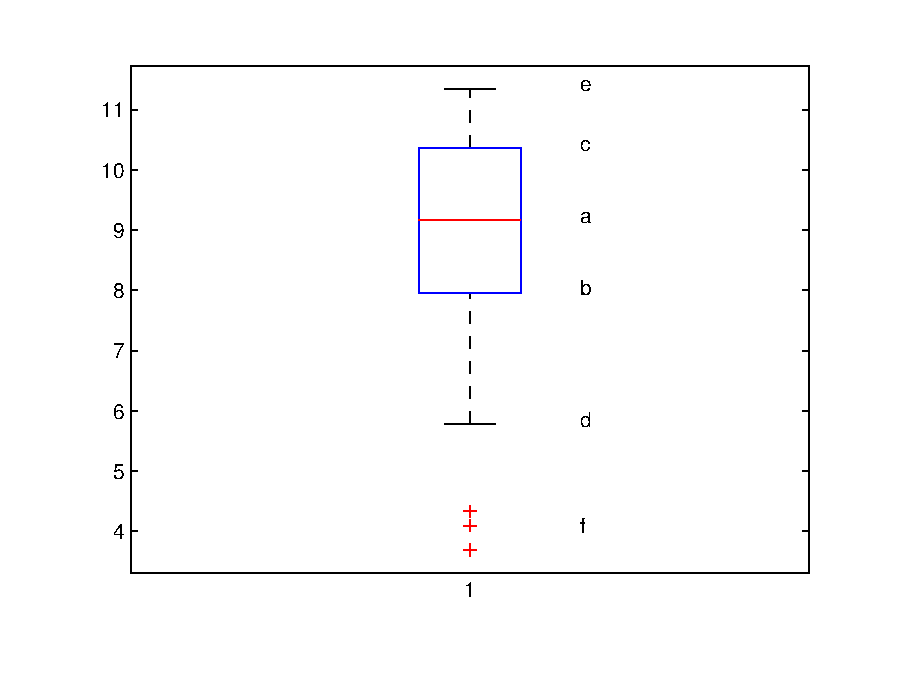
\includegraphics{figures/boxplot.eps}}
\end{center}
\vspace{-3em}
\caption{Boxplot}
\end{figure}
%a: empirischer Median, b: empirisches $0.25$-Quantil, c: empirisches $0.75$-Quantil, d: kleinster Datenwert $x_i$ mit $b-x_i < 1.5 (c-b)$, e: gr�sster Datenwert $x_i$ mit $x_i - c < 1.5 (c-b)$.


% ------------------------------------------------------------------------------------------------ %
% QQ-PLOT
% ------------------------------------------------------------------------------------------------ %


\subsection{QQ-Plot}

Mit einem \emph{QQ-Plot} (Quantil-Quantil) kann man die Abweichung der Daten von einer gew�hlten Modell-Verteilung $F$ graphisch �berpr�fen.

Es werden die empirischen Quantile auf der $y$-Achse gegen�ber den theoretischen Quantilen auf der $x$-Achse geplottet.


% ------------------------------------------------------------------------------------------------ %
% ------------------------------------------------------------------------------------------------ %
% SCH�TZER
% ------------------------------------------------------------------------------------------------ %


\section{Sch�tzer}

F�r eine Stichprobe $X_1, \ldots, X_n$ soll ein passendes Modell gefunden werden. Die Parameter $\theta = (\theta_1, \ldots,\theta_m)$ des Modells versucht man mit einem \emph{Sch�tzer} $T = (T_1,\ldots,T_m)$ aufgrund der Stichprobe herauszufinden. Die Sch�tzer sind Zufallsvariablen der Form $T_j = t_j(X_1,\ldots,X_n)$ f�r eine geeignete Funktion $t_j:\R^n\rightarrow\R$. Durch Einsetzen von Daten $x_i$ erh�lt man \emph{Sch�tzwertwerte} $t_j(x_1,\ldots,x_n)$ f�r $\theta_j$.


\begin{definition}[Erwartungstreu]
Ein Sch�tzer $T$ heisst \emph{erwartungstreu} f�r $\theta$, falls $\E[T] = \theta$ (im Mittel wird richtig gesch�tzt).
\end{definition}

\begin{definition}[Konsistent]
Eine Folge von Sch�tzern $T^{(n)}, n\in\mathbb{N}$ heisst \emph{konsistent} f�r $\theta$, falls $T^{(n)}$ f�r $n \rightarrow \infty$ im Modell $\mathbb{P_\theta}$ gegen $\theta$ konvergiert. Das heisst f�r jedes $\theta \in \Theta$ und $\epsilon > 0$ gilt
$$
\lim_{n\rightarrow\infty} \mathbb{P}[\,\abs{T^{(n)}-\theta}>\epsilon\,] = 0.
$$
\end{definition}

\begin{note}
Der Grundraum $\Omega$ und die Menge der beobachtbaren Ereignisse $\mathcal{F}$ sind fest. Die Wahl des Parameters $\theta$ aus dem Parameterraum $\Theta$ hat aber Einfluss auf das Wahrscheinlichkeitsmass $\P_\theta$. Mit $\E_\theta$ wird der Erwartungswert unter $\P_\theta$ bezeichnet.
\end{note}


% ------------------------------------------------------------------------------------------------ %
% MOMENTEN METHODE
% ------------------------------------------------------------------------------------------------ %


\subsection{Momenten-Methode}

\begin{definition}[Moment]
Das \emph{$k$-te Moment} einer Zufallsvariablen $X$ im Model $\P_\theta$ ist
$$
\mu_k := \mu_k(\theta) := \E_\theta[X^k].
$$
\end{definition}

\begin{definition}[Stichprobenmoment]
Das \emph{$k$-te Stichprobenmoment} von Zufallsvarialben $X_1,\ldots,X_n$ ist
$$
\hat\mu_k := \frac{1}{n} \sum_{i=1}^n X_i^k.
$$
\end{definition}

Die Parameter $\theta_i$ der theoretischen Verteilung werden als Funktion der Momente $\mu_k$ angegeben.
$$
\theta_j = g_j (\mu_1,\ldots,\mu_m)
\quad\text{f�r }j \in \{1,\ldots,m\}
$$
Den \emph{Momentensch�tzer} f�r $\theta = (\theta_1,\ldots,\theta_m)$ erh�lt man, indem man die Stichprobenmomente in die Funktionen der Momente einsetzt; der Sch�tzer ist also $T 
= (T_1,\ldots,T_m)$ mit
$$
T_j := g_j(\hat\mu_1,\ldots,\hat\mu_m)
\quad\text{f�r }j \in \{1,\ldots,m\}
$$

\begin{example}
Gegeben seien $n$ unabh�ngige Realisierungen $x_1,\ldots,x_n$ einer Zufallsvariablen $X \sim \mathcal{P}(\lambda)$. Es gilt $\E[X] = \lambda$. F�r die Funktion $g_1$ kann also die Idendit�t gew�hlt werden. Der Momentensch�tzer ist somit
$$
\lambda_\text{MM} = \hat\mu_1 = \frac{1}{n} \sum_{i=1}^n x_i = \overline{x}.
$$
Es gilt aber auch $\var[X] = \E[X^2]-\E[X]^2 = \lambda$. Es kann also auch $g_1(\mu_1,\mu_2) = \mu_2-\mu_1^2$ gew�hlt werden. Dadurch erh�lt man einen anderen Momentensch�tzer
$$
\lambda_\text{MM} =
\left(\frac{1}{n} \sum_{i=1}^n x_i^2\right) - \left(\sum_{i=1}^n x_i\right)^2 =
\frac{1}{n} \sum_{i=1}^n (x_i - \overline{x})^2
$$
\end{example}


% ------------------------------------------------------------------------------------------------ %
% MAXIMUM LIKELIHOOD
% ------------------------------------------------------------------------------------------------ %


\subsection{Maximum-Likelihood}

Es wird von einer Zufallsvariable $X_1,\ldots,X_n$ ausgegangen, deren gemeinsame Dichte $f(t_1,\ldots,t_n \mid \theta)$ von einem Parameter $\theta$ abh�ngt.
Die \emph{Likelihood-Funktion} $\mathcal{L}$ ist gegeben durch
$$
\mathcal{L}(x_1,\ldots,x_n \mid \theta) =
f(x_1,\ldots,x_n \mid \theta).
$$
Anschaulich ist das die Wahrscheinlichkeit\footnote{oder zumindest das stetige Pendant zur Wahrscheinlichkeit.}, dass im Modell $\P_\theta$ die Stichprobe $X_1,\ldots,X_n$ die Werte $x_1,\ldots,x_n$ liefert.
Um eine m�glichst gute Anpassung des Modells an die Daten zu erreichen, wird der Likelihood-Sch�tzer als Funktion von $\theta$ maximiert.

\begin{note}
Im diskreten Fall wird lediglich die Dichte $f$ durch die Gewichtsfunktion $p$ ersetzt.
\end{note}

Oft sind die Zufallsvariablen $X_i$ unter $\P_\theta$ i.i.d. mit Dichtefunktion $f(t \mid \theta)$, so dass sich die Likelihood-Funktion vereinfacht zu
$$
\mathcal{L}(x_1,\ldots,x_n \mid \theta) =
\prod_{i=1}^n f(x_i \mid \theta).
$$
Aufgrund der Monotonie des Logarithmus kann dann die logarithmierte Likelihood-Funktion verwendet werden, ohne dass sich dadurch das Maximum der Funktion verschiebt.
$$
\log \mathcal{L}(x_1,\ldots,x_n \mid \theta) =
\sum_{i=1}^n \log f(x_i \mid \theta)
$$


\begin{example}
Gegeben seien $n$ unabh�ngige Realisierungen  $x_1,\ldots,x_n$ einer Zufallsvariable $X \sim Exp(\lambda)$ mit Dichte
$f(t) = \lambda e^{-\lambda t} \mathbb{1}_{[0,\infty)}(t)$ und unbekanntem Parameter $\lambda$.
F�r die Likelihood-Funktion erh�lt man
$$
\mathcal{L}(\lambda) := \mathcal{L}(x_1,\ldots,x_n \mid \lambda) =
\prod_{i=1}^n \lambda e^{-\lambda x_i}
$$
und durch logarithmieren
$$
\log\mathcal{L}(\lambda) =
\sum_{i=1}^n \log \lambda e^{-\lambda x_i} =
n \log \lambda - \lambda \sum_{i=1}^n x_i.
$$
Zur Bestimmung des Maximums wird die Ableitung nullgesetzt:
$$
\frac{\d}{\d\lambda}\log\mathcal{L}(\lambda) =
\frac{n}{\lambda} - \sum_{i=1}^n x_i \overset{!}{=} 0
\quad\Rightarrow\quad
\lambda_\text{LH} = \frac{n}{\sum_{i=1}^n x_i}
$$
Aus $\frac{\d^2}{\d\lambda^2} \mathcal{L}(\lambda) = -\frac{n}{\lambda^2} < 0$ f�r $\lambda > 0$ folgt, dass es sich auch tats�chlich um ein Maximum handelt.
\end{example}


% ------------------------------------------------------------------------------------------------ %
% ------------------------------------------------------------------------------------------------ %
% TESTS
% ------------------------------------------------------------------------------------------------ %


\section{Tests}

\subsection{Fehler 1. und 2. Art}

\begin{definition}[Fehler 1. Art] Die Hypothese wird zu Unrecht abgelehnt, d.h. obwohl sie richtig ist. Die Wahrscheinlichkeit f�r einen Fehler 1. Art ist
$$
\P_\theta[T \in K]
\quad\text{f�r } \theta \in \Theta_0.
$$
\end{definition}

\begin{definition}[Fehler 2. Art]
Die Hypothese wird akzeptiert, obwohl sie falsch ist. Die Wahrscheinlichkeit f�r einen Fehler 2. Art ist
$$
\P_\theta[T \notin K] =
1 - \P_\theta[T \in K]
\quad\text{f�r } \theta \in \Theta_A.
$$
\end{definition}


% ------------------------------------------------------------------------------------------------ %
% M�GLICHES VORGEHEN
% ------------------------------------------------------------------------------------------------ %


\subsection{M�gliches Vorgehen}

Ausgangspunkt ist eine Stichprobe $X_1,\ldots,X_n$ in einem Modell $\P_\theta$ mit unbekanntem Parameter $\theta \in \Theta$.

\begin{compactenum}[1:]
\item
Aufgrund einer Vermutung, wo sich der richtige Parameter $\theta$ befindet, werden eine \emph{Hypothese} $\Theta_0 \subseteq \Theta$ und eine \emph{Alternative} $\Theta_A \subseteq \Theta$ mit $\Theta_0 \cap \Theta_A = \emptyset$ formuliert:
\begin{center}
\vspace{1ex}
\begin{tabular}{r@{ : }l}
Hypothese $H_0$ & $\theta \in \Theta_0$ \\
Alternative $H_A$ & $\theta \in \Theta_A$
\end{tabular}
\end{center}
\end{compactenum}

\begin{note}
Die Hypotese (bzw. Alternative) heisst \emph{einfach}, falls sie nur aus einem einzelnen Wert besteht, also z.B. $\Theta_0 = \{\theta_0\}$ (bzw. $\Theta_A = \{\theta_A\})$.
\end{note}

\begin{compactenum}
\setcounter{enumi}{1}
\item
Es wird eine \emph{Teststatistik} $T = t (X_1,\ldots,X_n)$ gew�hlt, wobei $t:\R^n\rightarrow\R$ eine geeignete Funktion ist.

\item
Es wird ein \emph{Signifikanzniveau} $\alpha \in (0,1)$ gew�hlt.

\item Ein \emph{Verwerfungsbereich} $K \subseteq \R$ wird konstruiert, so dass
$$
\sup_{\theta \in \Theta_0} \P_\theta[T \in K] \leq \alpha.
$$
Dadurch wird die Wahrscheinlichkeit eines Fehlers 1. Art durch $\alpha$ beschr�nkt.

\item
Die Hypothese wird verworfen, falls der realisierte Wert $t(x_1,\ldots,x_n)$ im Verwerfungsbereich $K$ liegt.
\end{compactenum}

\begin{note}
Alternative zu Schritt 4 und 5:
Der P-Wert $p$ wird berechnet und die Hypothese verworfen, falls $p \leq \alpha$.
\end{note}

\begin{definition}[P-Wert]
Der P-Wert ist die Wahrscheinlichkeit, dass unter der Nullhypothese $H_0$ ein zuf�lliger Versuch mindestens so extrem ausf�llt, wie der beobachtete Wert $t$.
\end{definition}

\begin{definition}[Macht]
Die \emph{Macht} eines Tests ist die Funktion
$$
\beta:\Theta_A\rightarrow[0,1],\quad
\theta \mapsto\beta(\theta) := \mathbb{P}_\theta[T \in K].
$$
Das Maximieren der Macht $\beta(\theta)$ entspricht dem Minimieren der Wahrscheinlichkeit f�r einen Fehler 2. Art $1-\beta(\theta) = \mathbb{P}_\theta[T\notin K]$ f�r $\theta \in \Theta_A$.
\end{definition}


% ------------------------------------------------------------------------------------------------ %
% LIKELIHOOD QUOTIENT
% ------------------------------------------------------------------------------------------------ %


\subsection{Likelihood-Quotienten Test}

Als Teststatistik wird der \emph{Likelihood-Quotient} $\mathcal{R}$ gew�hlt, wobei $\mathcal{L}$ die Likelihood-Funktion ist:
$$
T :=
\mathcal{R}(x_1,\ldots,x_n) :=
\frac
  {\displaystyle\sup_{\theta\in\Theta_0}\mathcal{L}(x_1,\ldots,x_n \mid \theta)}
  {\displaystyle\sup_{\theta\in\Theta_A}\mathcal{L}(x_1,\ldots,x_n \mid \theta)}
$$
Ist dieser Quotient klein, sind die Beobachtungen im Modell $\P_{\Theta_A}$ deutlich wahrscheinlicher als im Modell $\P_{\Theta_0}$. Der Verwerfungsbereich $K := [0,c)$ wird so gew�hlt, dass der Test das gew�nschte Signifikanzniveau einh�lt.

\begin{note}
Sind Hypothese und Alternative beide einfach, so ist der Test optimal (nach Neyman-Pearson-Lemma).
\end{note}


% ------------------------------------------------------------------------------------------------ %
% Z-TEST
% ------------------------------------------------------------------------------------------------ %


\subsection{z-Test}

%Normalverteilung, Test f�r Erwartungswert bei bekannter Varianz:
Seien $X_1,\ldots,X_n \overset{i.i.d.}{\sim} \mathcal{N}(\theta_0,\sigma^2)$ unter $\P_{\theta_0}$ mit \emph{bekannter} Varianz $\sigma^2$. Es soll die Hypothese $H_0: \theta = \theta_0$ getestet werden. M�gliche Alternativen $H_A$ sind $\theta > \theta_0$, $\theta < \theta_0$ (einseitig) oder $\theta \neq \theta_0$ (zweiseitig). Die Teststatistik ist
$$
T := \frac{\overline{X}_n - \theta_0}{\sigma_X / \sqrt{n}} \sim \mathcal{N}(0,1)
$$
unter dem Modell $\P_{\theta_0}$.  Der Verwerfungsbereich ist von der Form $(c_>,\infty)$, bzw. $(-\infty,c_<)$, bzw. $(-\infty,-c_{\neq})\cup(c_{\neq},\infty)$. Zum Beispiel liefert die Bedingung
$$
\alpha =
\P_{\theta_0}[T \in K_>] =
\P_{\theta_0}[T > c_>] =
1- \Phi(c_>),
$$
dass $c_> = \Phi^{-1}(1-\alpha)$, also das $(1-\alpha)$-Quantil der $\mathcal{N}(0,1)$-Verteilung, sein muss.


% ------------------------------------------------------------------------------------------------ %
% T-TEST
% ------------------------------------------------------------------------------------------------ %


\subsection{t-Test}

%Normalverteilung, Test f�r Erwartungswert bei unbekannter Varianz:
Seien $X_1,\ldots,X_n \overset{\text{i.i.d.}}{\sim} \mathcal{N}(\mu_0,\sigma^2)$ unter $\P_\theta$ wobei $\theta = (\mu,\sigma^2)$ und insbesondere die Varianz $\sigma^2$ \emph{unbekannt} ist. Die Hypothese $H_0: \mu = \mu_0$ soll getestet werden.
Die unbekannte Varianz $\sigma^2$ wird durch den Sch�tzer $s^2 = \frac{1}{n-1} \sum_{i=1}^n (X_i-\overline{X})^2$ (empirische Varianz) ersetzt. Danach kann mit der Teststatistik
$$
T := \frac{\overline{X}_n - \mu_0}{s / \sqrt{n}} \sim t_{n-1}
$$
gleich wie beim z-Test vorgegangen werden.


% ------------------------------------------------------------------------------------------------ %
% GEPAARTE ZWEISTICHPROBEN TESTS
% ------------------------------------------------------------------------------------------------ %


\subsection{Gepaarter Zweistichprobentest}

Seien $X_{1\leq i \leq n} \overset{\text{i.i.d.}}{\sim} \mathcal{N}(\mu_X,\sigma^2)$ und $Y_{1\leq i \leq n} \overset{\text{i.i.d.}}{\sim} \mathcal{N}(\mu_Y,\sigma^2)$ unter $\P_\theta$. Falls man eine nat�rliche Paarbildung zwischen $X_i$ und $Y_i$ hat, l�sst der Test zum Vergleich von $\mu_X$ und $\mu_Y$ auf eine Stichprobe zur�ckf�hren:
$$
Z_i := X_i - Y_i
\overset{\text{i.i.d.}}{\sim}
\mathcal{N}(\mu_x-\mu_y,2\sigma^2)
$$

\subsection{Ungepaarter Zweistichprobentest}

Seien $X_{1\leq i \leq n} \overset{\text{i.i.d.}}{\sim} \mathcal{N}(\mu_X,\sigma^2)$ und $Y_{1\leq i \leq m} \overset{\text{i.i.d.}}{\sim} \mathcal{N}(\mu_Y,\sigma^2)$ unter $\P_\theta$.

\begin{compactenum}[\bf a)]
\item
	Ist $\sigma^2$ bekannt, so ist die Teststatistik
	$$
	T := \frac{(\overline{X}_n-\overline{Y}_m)-(\mu_X-\mu_Y)}{\sigma\sqrt{\frac{1}{n}+\frac{1}{m}}} \sim \mathcal{N}(0,1).
	$$
\item
	Ist $\sigma^2$ unbekannt, berechnet man
	$$
	s^2 := \frac{1}{m+n-2}((n-1)s_X^2+(m-1)s_Y^2)
	$$
	und w�hlt f�r die Teststatistik
	$$
	T := \frac{(\overline{X}_n-\overline{Y}_m)-(\mu_X-\mu_Y)}{s\sqrt{\frac{1}{n}+\frac{1}{m}}} \sim t_{n+m-2}
	$$
\end{compactenum}


% ------------------------------------------------------------------------------------------------ %
% VERTRAUENSINTERVALL
% ------------------------------------------------------------------------------------------------ %


\subsection{Konfidenzbereiche}

\begin{definition}[Konfidenzbereich]
Ein \emph{Konfidenzbereich} f�r $\theta$ zu den Stichproben $X_1,\ldots,X_n$ ist eine Menge $C(X_1,\ldots,X_n) \subseteq \Theta$. In den meisten F�llen ist das ein Intervall, dessen Endpunkte von $X_1,\ldots,X_n$ abh�ngen.

$C$ heisst ein Konfidenzbereich zum \emph{Niveau} $1-\alpha$, falls gilt
$$
\P_\theta[\theta \in C(X_1,\ldots,X_n)] \geq 1-\alpha
$$
\end{definition}


% ------------------------------------------------------------------------------------------------ %

{\Large Mit 💖 gemacht von Max Mathys 👊}

\vspace{.7em}

\textbf{Schule}: MNG Rämibühl
\vspace{.2em}

\textbf{Jahr}: 2016
\vspace{.2em}

\textbf{Lehrerin}: Antoniadis	

\label{lastpage}

\end{document}


% ------------------------------------------------------------------------------------------------ %